\documentclass{article}
\usepackage[T1]{fontenc}
\usepackage{lmodern}
\usepackage{graphicx}
\usepackage{amsmath,amssymb}
\usepackage[a4paper,margin=2cm]{geometry}
\usepackage[absolute,overlay]{textpos}
\setlength{\TPHorizModule}{1mm}
\setlength{\TPVertModule}{1mm}
\usepackage[indonesian]{babel}
\usepackage{hyperref}
\setlength{\emergencystretch}{2em}
% unit: Halaman 20

\begin{document}

% === Halaman 20 (python/native) ===

• E adalah fungsi ekspansi yang memperluas blok Ri – 1 

32-bit menjadi blok 48 bit. 

• Fungsi ekspansi direalisasikan dengan matriks 

permutasi ekspansi:

32 

1 

2 

3 

4 

5 

4 

5 

6 

7 

8 

9 

8 

9 

10 

11 

12 

13 

12 

13 

14 

15 

16 

17 

16 

17 

18 

19 

20 

21 

20 

21 

22 

23 

24 

25 

24 

25 

26 

27 

28 

29 

28 

29 

30 

31 

32 

1 


20

% deskripsi: gambar native xref 116
\noindent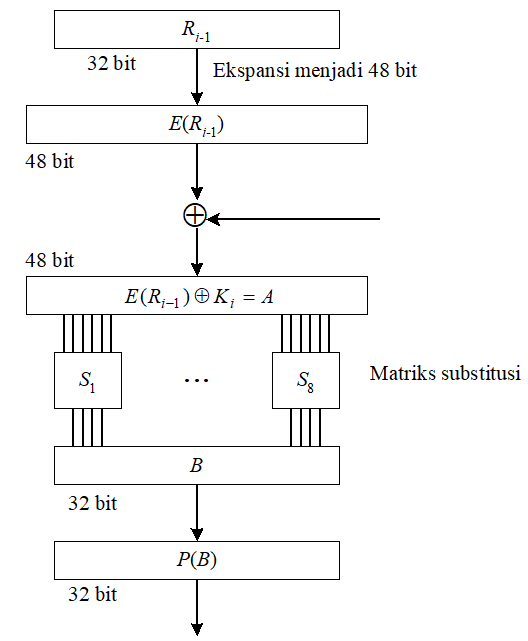
\includegraphics[width=0.85\textwidth]{../../images/python/page_020_img_01.png}

\end{document}
